
\subsection{Subsystem 1 grasping subsystem}

\begin{figure}[h!]
	\centering
 	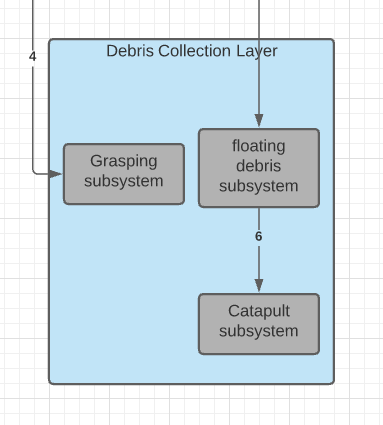
\includegraphics[width=0.60\textwidth]{images/subsystem_debris}
 \caption{Example subsystem description diagram}
\end{figure}

\subsubsection{Assumptions}
Since the debris collection is clearly spelled out in the competition instructions, no assumptions are necessary for this subsystem.

\subsubsection{Responsibilities}
Grab the underwater debris, be able to hold onto the debris while the submarine is navigating through water with water resistance pushing the block, and then release the debris in the deposit location.

\subsubsection{Subsystem Interfaces}

\begin {table}[H]
\caption {Subsystem interfaces} 
\begin{center}
    \begin{tabular}{ | p{1cm} | p{6cm} | p{3cm} | p{3cm} |}
    \hline
    ID & Description & Inputs & Outputs \\ \hline
    \#xx & Description of the interface/bus & \pbox{3cm}{input 1 \\ input 2} & \pbox{3cm}{output 1}  \\ \hline
    \#xx & Description of the interface/bus & \pbox{3cm}{N/A} & \pbox{3cm}{output 1}  \\ \hline
    \end{tabular}
\end{center}
\end{table}

\subsection{Subsystem 2 floating debris subsystem}
\subsubsection{Assumptions}
Since the debris collection is clearly spelled out in the competition instructions, no assumptions are necessary for this subsystem.

\subsubsection{Responsibilities}
collect debris floating on top of the water and deposit it in the catapult system. This will be done kinetically so there are no inputs to this mechanism.

\subsubsection{Subsystem Interfaces}

\begin {table}[H]
\caption {Subsystem interfaces} 
\begin{center}
	\begin{tabular}{ | p{1cm} | p{6cm} | p{3cm} | p{3cm} |}
		\hline
		ID & Description & Inputs & Outputs \\ \hline
		\#xx & Description of the interface/bus & \pbox{3cm}{input 1 \\ input 2} & \pbox{3cm}{output 1}  \\ \hline
		\#xx & Description of the interface/bus & \pbox{3cm}{N/A} & \pbox{3cm}{output 1}  \\ \hline
	\end{tabular}
\end{center}
\end{table}

\subsection{Subsystem 3}
\subsection{Subsystem 2 catapult subsystem}
\subsubsection{Assumptions}
We assumed it will be necessary to launch the debris up a little bit in order to get it over the lip of the deposit station.

\subsubsection{Responsibilities}
launch the floating debris that we collected into the deposit station.

\subsubsection{Subsystem Interfaces}

\begin {table}[H]
\caption {Subsystem interfaces} 
\begin{center}
	\begin{tabular}{ | p{1cm} | p{6cm} | p{3cm} | p{3cm} |}
		\hline
		ID & Description & Inputs & Outputs \\ \hline
		\#xx & Description of the interface/bus & \pbox{3cm}{input 1 \\ input 2} & \pbox{3cm}{output 1}  \\ \hline
		\#xx & Description of the interface/bus & \pbox{3cm}{N/A} & \pbox{3cm}{output 1}  \\ \hline
	\end{tabular}
\end{center}
\end{table}

